\titleframe

% Contoh Kode Slide
%\section{Introduction}
%\begin{frame}{\insertsectionhead}
%	\framesubtitle{A short introduction to Trigon}
%	\themename is a modern, elegant and versatile theme for Beamer, inspired by
%	the
%	\href{https://github.com/matze/mtheme}{\textsc{metropolis} theme} from Matthias
%	Vogelgesang.
%	\vfill
%	\themename comes with lots of nice extra features
%	\begin{itemize}
%		\item Multiple style variations for title, section and normal slides
%		\item Simple customization of theme colors
%		\item Lots of convenient options to tweak the design
%	\end{itemize}
%\end{frame}

% Contoh Kode Tabel
%  \begin{table}[H]
% \centering
% \caption{A nice table example}
% \begin{tabular}{@{} lccc @{}}
%    \toprule
%    & \textbf{Velocity} & \textbf{Angle}  & \textbf{Vertical force} \\
%    & $U$ & $\alpha$  & $F_z$ \\
%    & [m/s] & [$^\circ$]  & [N] \\
%    \midrule
%    2D simulation  & 9 & 2 & 9.23 \\
%    3D simulation  & 10.0 & 3 & 15.039 \\
%    Experiment A   & 11.31 & 2.5 & 13.2 \\
%    Experiment B   & 11.26 & 2.7 & 12.6 \\
%    Experiment C   & 11.33 & 2.47 & 13.6 \\
%    \bottomrule
%  \end{tabular}
%\end{table}

% Contoh Kode Gambar
%  \begin{figure}[ht!]
%	\begin{subfigure}[b]{0.3\textwidth}
%		\frame{\includegraphics[width=\textwidth]{layout_example-03.jpg}}
%		\caption*{plain}
%	\end{subfigure}
%	\hspace{\fill}
%	\begin{subfigure}[b]{0.3\textwidth}
%		\frame{\includegraphics[width=\textwidth]{layout_example-02.jpg}}
%		\caption*{style1}
%	\end{subfigure}
%	\hspace{\fill}
%	\begin{subfigure}[b]{0.3\textwidth}
%		\frame{\includegraphics[width=\textwidth]{layout_example-01.jpg}}
%		\caption*{style2 (default)}
%	\end{subfigure}
%\end{figure}

% Contoh Kode Blocks
% \begin{block}{Regular block}
%	Just a regular block
%\end{block}
%\begin{alertblock}{Alert block}
%	Some important thing
%\end{alertblock}
%\begin{exampleblock}{Example block}
%	No difference with regular block to avoid excessive distraction
%\end{exampleblock}

\setbeamertemplate{frame footer}{Alauddin Maulana Hirzan, M. Kom - Universitas Semarang}

\section{Ketentuan Perkuliahan}
\begin{frame}{\insertsectionhead}
	\framesubtitle{Peraturan Dasar dan Ketentuan Lain}
	\justifying
	Mahasiswa \textbf{diwajibkan}:
	\begin{itemize}
		\item Datang tepat waktu
		\item Mengerjakan tugas, kegiatan, dan ujian tepat waktu
		\item Rajin melakukan pengecekan nilai
		\item Aktif di dalam kelas
	\end{itemize}
	Dosen \textbf{diwajibkan}:
	\begin{itemize}
		\item Memberi materi perkuliahan
		\item Memberi penilaian dari tugas dan ujian
		\item Mengarahkan mahasiswa dalam praktikum
	\end{itemize}
\end{frame}

\begin{frame}{\insertsectionhead}
	\framesubtitle{Kontrak Penilaian}
	\justifying
	Dosen memberikan nilai dalam format nilai sebagai berikut:
	 \begin{table}[H]
	 \centering
	 \begin{tabular}{@{} lccc @{}}
		    \toprule
		   \textbf{Kategori} & \textbf{Persentase} & \textbf{Keterangan} \\
		    \midrule
		    Presensi  & 10\% & Maks 10\% \\
		    Tugas  & 20\% & Lengkap \> Tidak Lengkap \\
		    Ujian Tengah   & 35\% & - \\
		    Ujian Akhir   & 35\% & - \\
		    \bottomrule
		  \end{tabular}
	\end{table}
	\begin{block}{Info}
		Nilai di atas tidak pasti hingga mahasiswa menentukan persentasenya !
	\end{block}
\end{frame}

\section{\textit{Internet of Everything \& Internet of Things}}
\begin{frame}{\insertsectionhead}
  \framesubtitle{Apa itu IoE?}
  \justifying
  Berdasarkan \textbf{\textit{ioe.org}}:
  \vfill
  \begin{quote}
  	Internet of Everything (IoE) adalah interkoneksi tanpa batas dan koordinasi otonom dari sejumlah besar elemen dan sensor komputasi, entitas mati dan hidup, orang, proses, dan data melalui infrastruktur Internet.
  \end{quote}
	\vfill
   Berdasarkan \textbf{\textit{technopedia.com}}:
	\vfill	
  \begin{quote}
  	IOE didasarkan pada gagasan bahwa di masa depan, koneksi internet tidak akan terbatas pada laptop atau komputer desktop dan beberapa tablet, seperti pada dekade sebelumnya. Sebaliknya, mesin umumnya akan menjadi lebih pintar dengan memiliki lebih banyak akses ke data dan memperluas peluang jaringan.
  \end{quote}
\end{frame}

\begin{frame}{\insertsectionhead}
	\framesubtitle{Mengenal IoE}
	\justifying
	Bisa disimpulkan bahwa \textit{Internet of Everything} adalah sebuah teknologi yang di mana semua perangkat komputasi, entitas, orang, proses, dan data terhubung \textbf{satu sama lain} melalui infrastruktur Internet.
	\vfill
	\begin{block}{Contoh}
		Pengguna gawai cerdas yang terhubung ke Internet dapat menghidupkan lampu rumah maupun mengendalikan kendaraan pribadi tanpa harus berada di tempat tersebut.
	\end{block}
\end{frame}

\begin{frame}{\insertsectionhead}
	\framesubtitle{\textit{Advanced Summon Tesla}}
	\justifying
	\begin{figure}[ht!]
			\begin{subfigure}[b]{0.7\textwidth}
					\frame{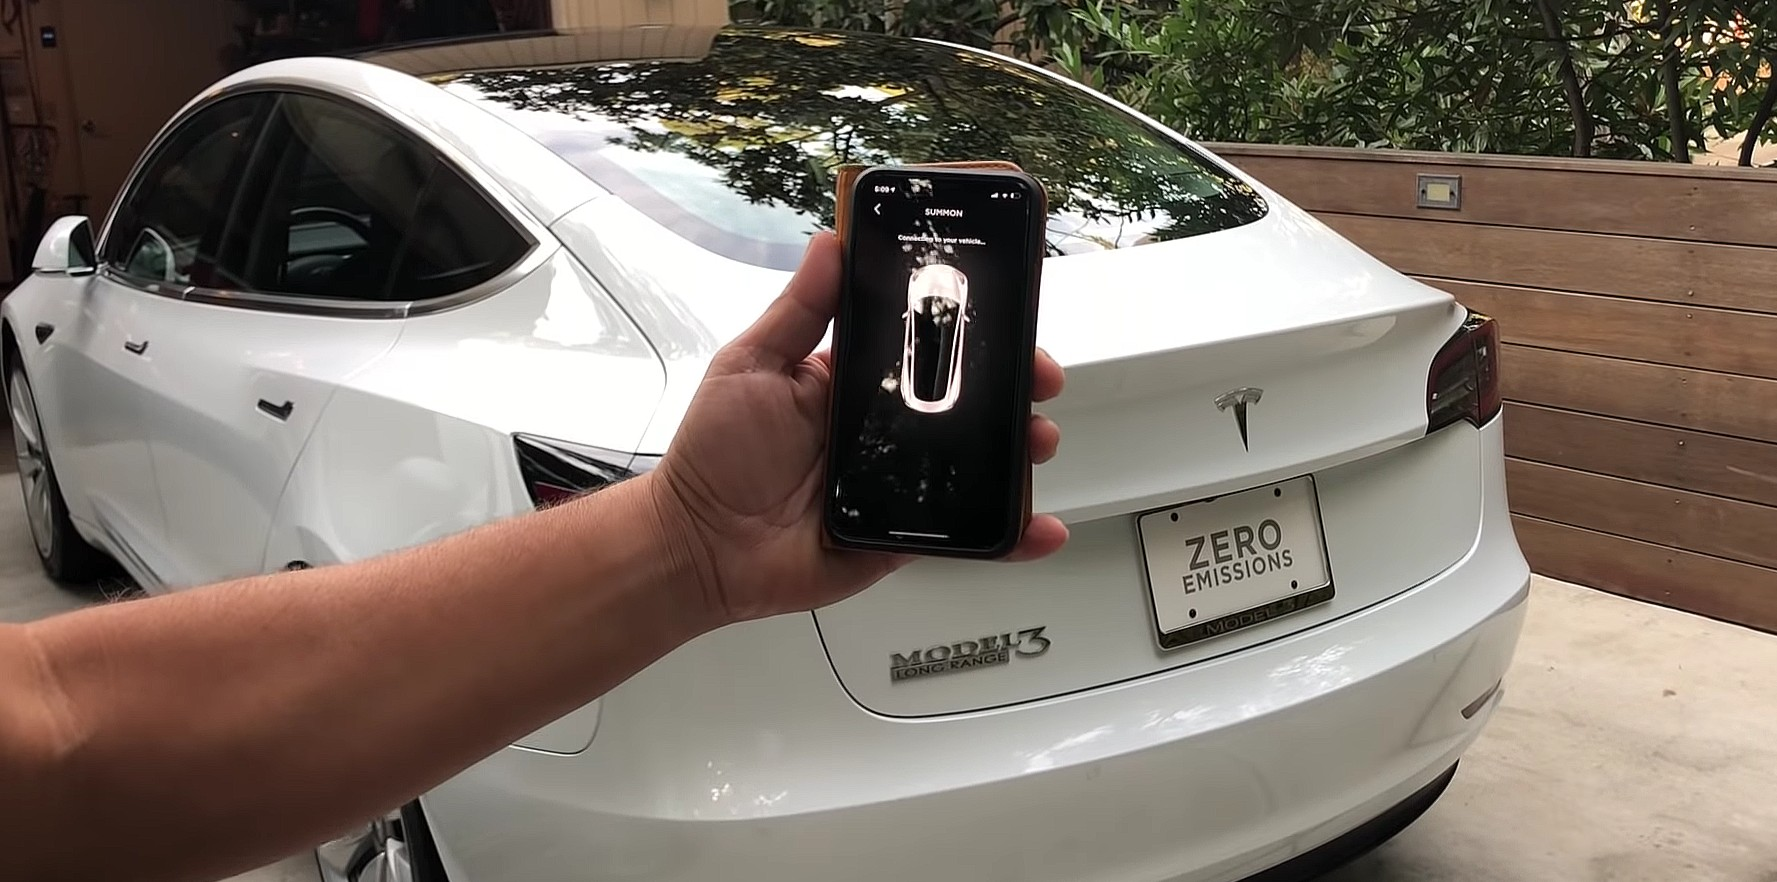
\includegraphics[width=\textwidth]{tesla-remote.jpg}}
					\caption*{Tesla dengan teknologi panggilan jarak jauh}
				\end{subfigure}
		\end{figure}
\end{frame}

\begin{frame}{\insertsectionhead}
	\framesubtitle{Tetapi?}
	\justifying
	\centering
	Teknologi ini masih secuil dari \textit{Internet of Everything}, sehingga belum layak dipanggil sebagai bagian dari teknologi tersebut. Dikarenakan terdapat beberapa elemen yang belum masuk di contoh tersebut.
	\vfill
	Teknologi bagian dari \textit{Internet of Everything} ini adalah \\
	\textbf{\textit{\large Internet of Things}}
\end{frame}

\begin{frame}{\insertsectionhead}
	\framesubtitle{Apa itu IoT?}
	\justifying
	Berdasarkan \textbf{\textit{NIST SP 800-172}}:
	\vfill
	\begin{quote}
		Jaringan perangkat yang berisi perangkat keras, perangkat lunak, firmware, dan aktuator yang memungkinkan perangkat terhubung, berinteraksi, dan bertukar data dan informasi secara bebas.
	\end{quote}
	\vfill
	Berdasarkan \textbf{\textit{Asghari, P., Rahmani, A. M., \& Javadi, H. H. S. (2019)}}:
	\vfill
	\begin{quote}
		Ekosistem yang berisi objek pintar yang dilengkapi dengan sensor, jaringan, dan teknologi pemrosesan yang terintegrasi dan bekerja sama untuk menyediakan layanan cerdas untuk pengguna akhir.
	\end{quote}
\end{frame}

\begin{frame}{\insertsectionhead}
	\framesubtitle{Contoh}
	\justifying
	\begin{figure}[ht!]
		\begin{subfigure}[b]{0.6\textwidth}
			\frame{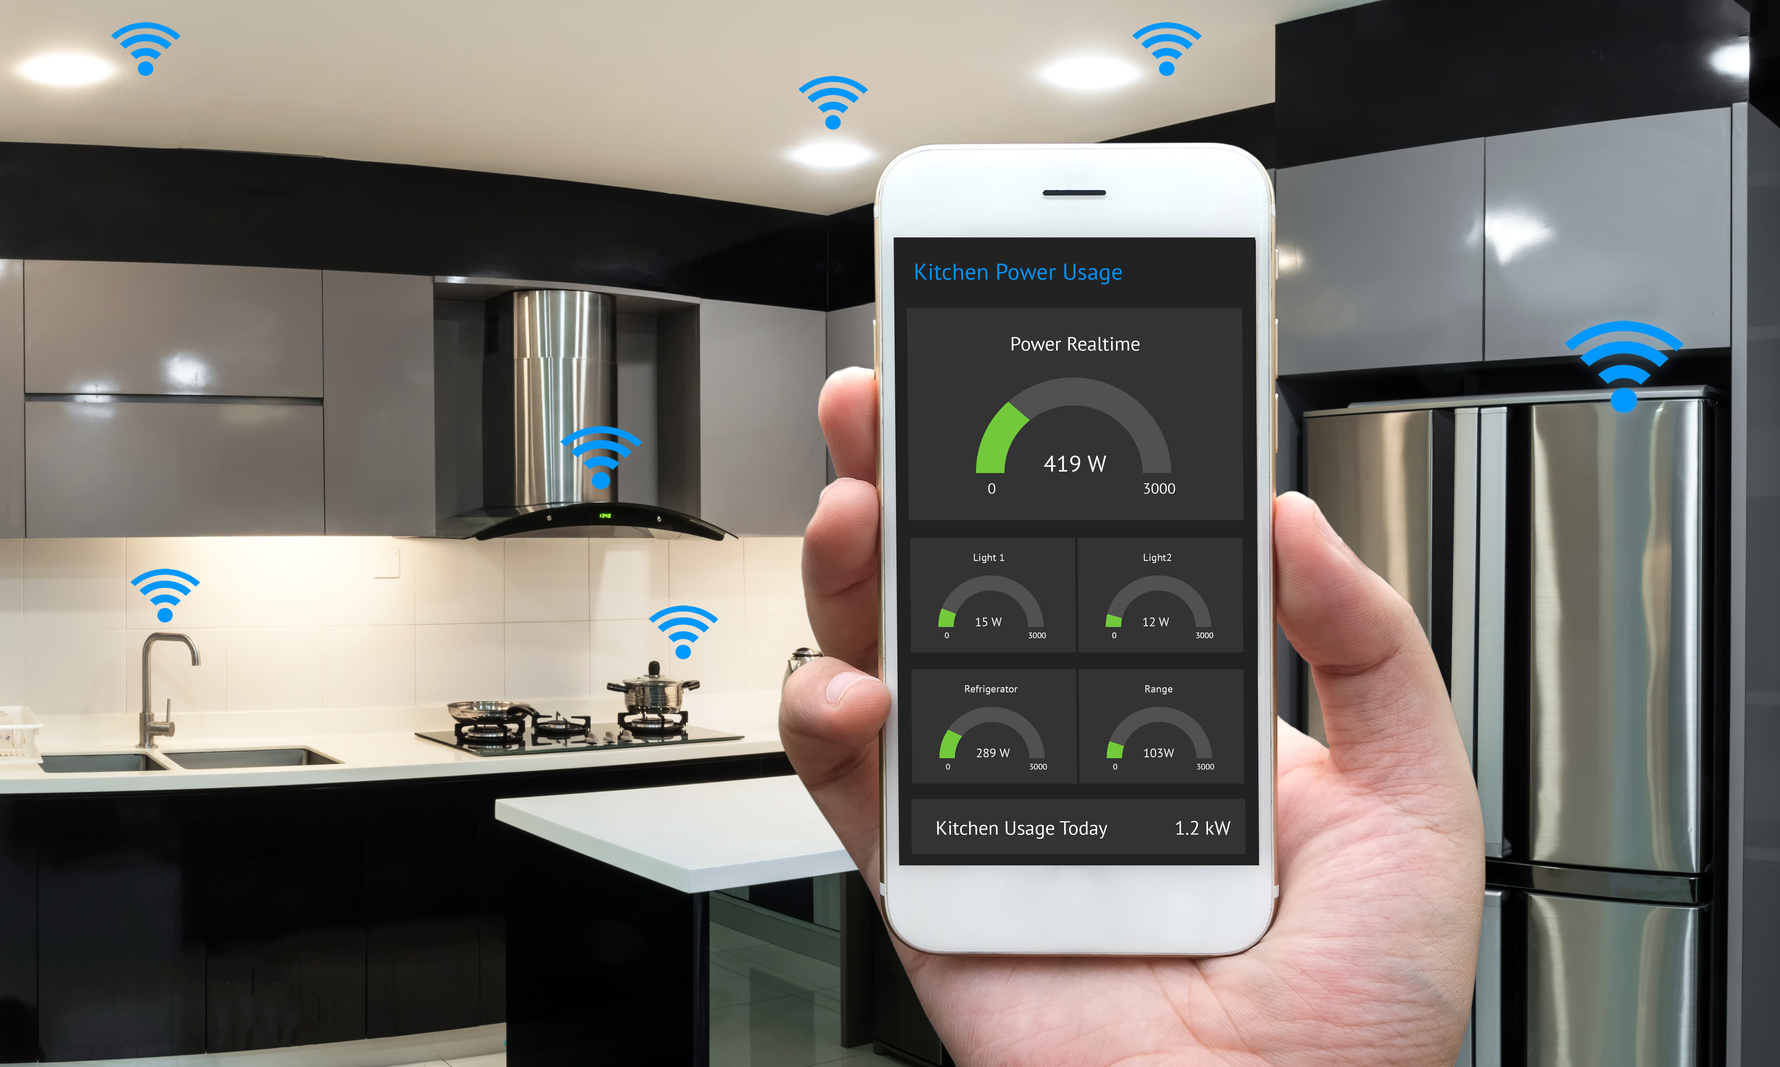
\includegraphics[width=\textwidth]{contoh-iot.jpg}}
			\caption*{Menggunakan IoT untuk memantau penggunaan daya listrik}
		\end{subfigure}
	\end{figure}
\end{frame}

\begin{frame}[fragile=singleslide]{\insertsectionhead}
	\framesubtitle{Cara Kerja \textit{Internet of Things}}
	\justifying
	Sistem IoT mengumpulkan dan menganalisis data terkini menggunakan sistem tertanam seperti prosesor, sensor, dan perangkat keras komunikasi. Perangkat ini berkomunikasi dengan perangkat lain yang terhubung dan bertindak berdasarkan informasi yang mereka terima dari satu sama lain.
	\begin{figure}[ht!]
		\begin{subfigure}[b]{0.6\textwidth}
			\frame{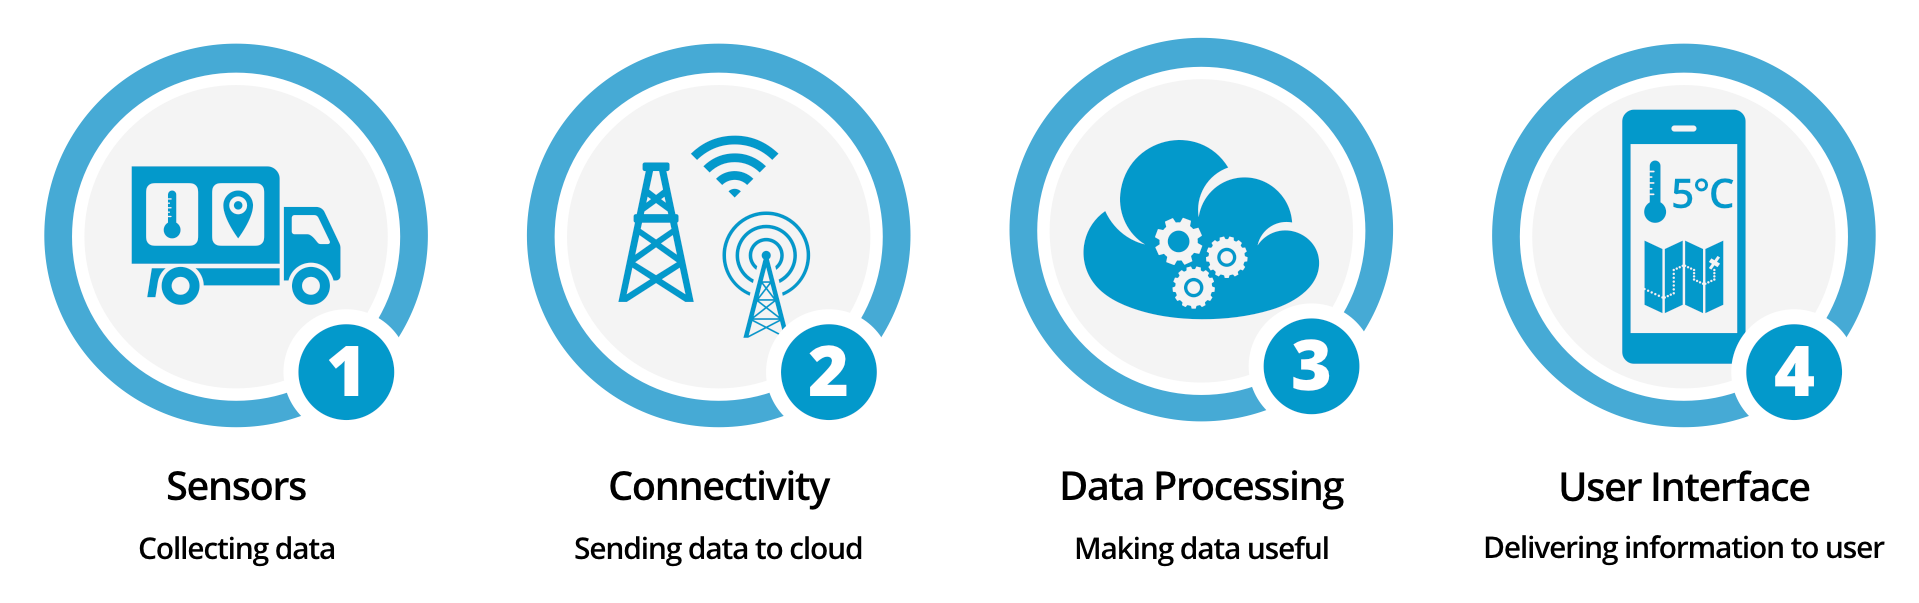
\includegraphics[width=\textwidth]{cara-kerja.png}}
			\caption*{IoT mengumpulkan, mengirim, dan menganalisis data}
		\end{subfigure}
	\end{figure}
\end{frame}

\begin{frame}[fragile=singleslide]{\insertsectionhead}
  \framesubtitle{Aplikasi Sederhana \textit{Internet of Things}}
  \justifying
  \textit{Internet of Things} dapat diimplementasikan dalam berbagai macam bentuk sesuai dengan kebutuhan pengguna. Selama komponen-komponen yang dibutuhkan tersedia, maka \textit{Internet of Things} dapat dibuat untuk mengatasi masalah tersebut.
  \vfill
  Sektor-sektor yang dapat didukung teknologi \textit{Internet of Things}:
  \begin{multicols}{2}
  \begin{itemize}
  	\item Kesehatan
  	\item Agraris
  	\item Maritim
  	\item Energi (Listrik)
  	\item Keuangan
  	\item Manufaktur/Produksi
  	\item Transpotasi/Logistik
  \end{itemize}
\end{multicols}
\end{frame}

\begin{frame}[fragile=singleslide]{\insertsectionhead}
	\framesubtitle{Aplikasi Kompleks \textit{Internet of Things}}
	\justifying
	\centering
	  \begin{figure}[ht!]
		\begin{subfigure}[b]{0.48\textwidth}
				\frame{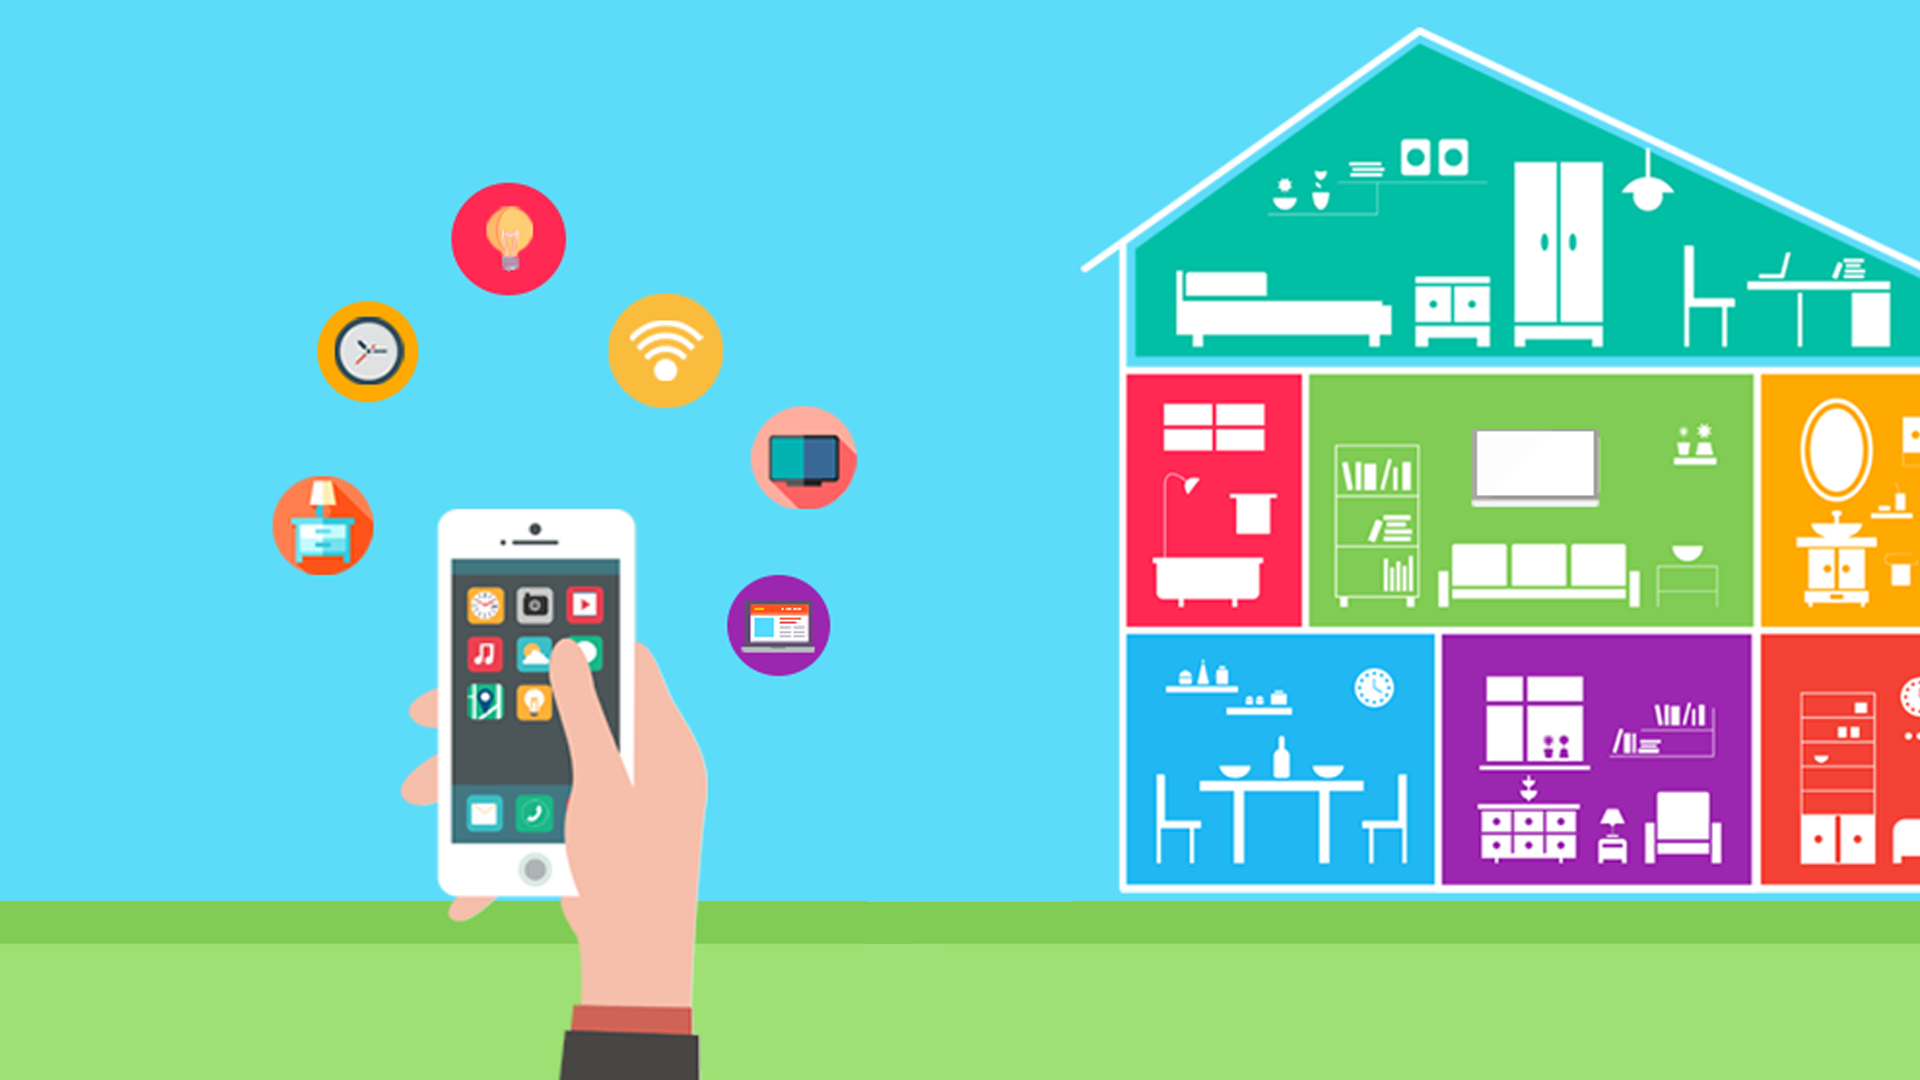
\includegraphics[width=\textwidth]{smarthome.png}}
				\caption*{\textit{Smart Home}}
			\end{subfigure}
		\hspace{\fill}
		\begin{subfigure}[b]{0.48\textwidth}
				\frame{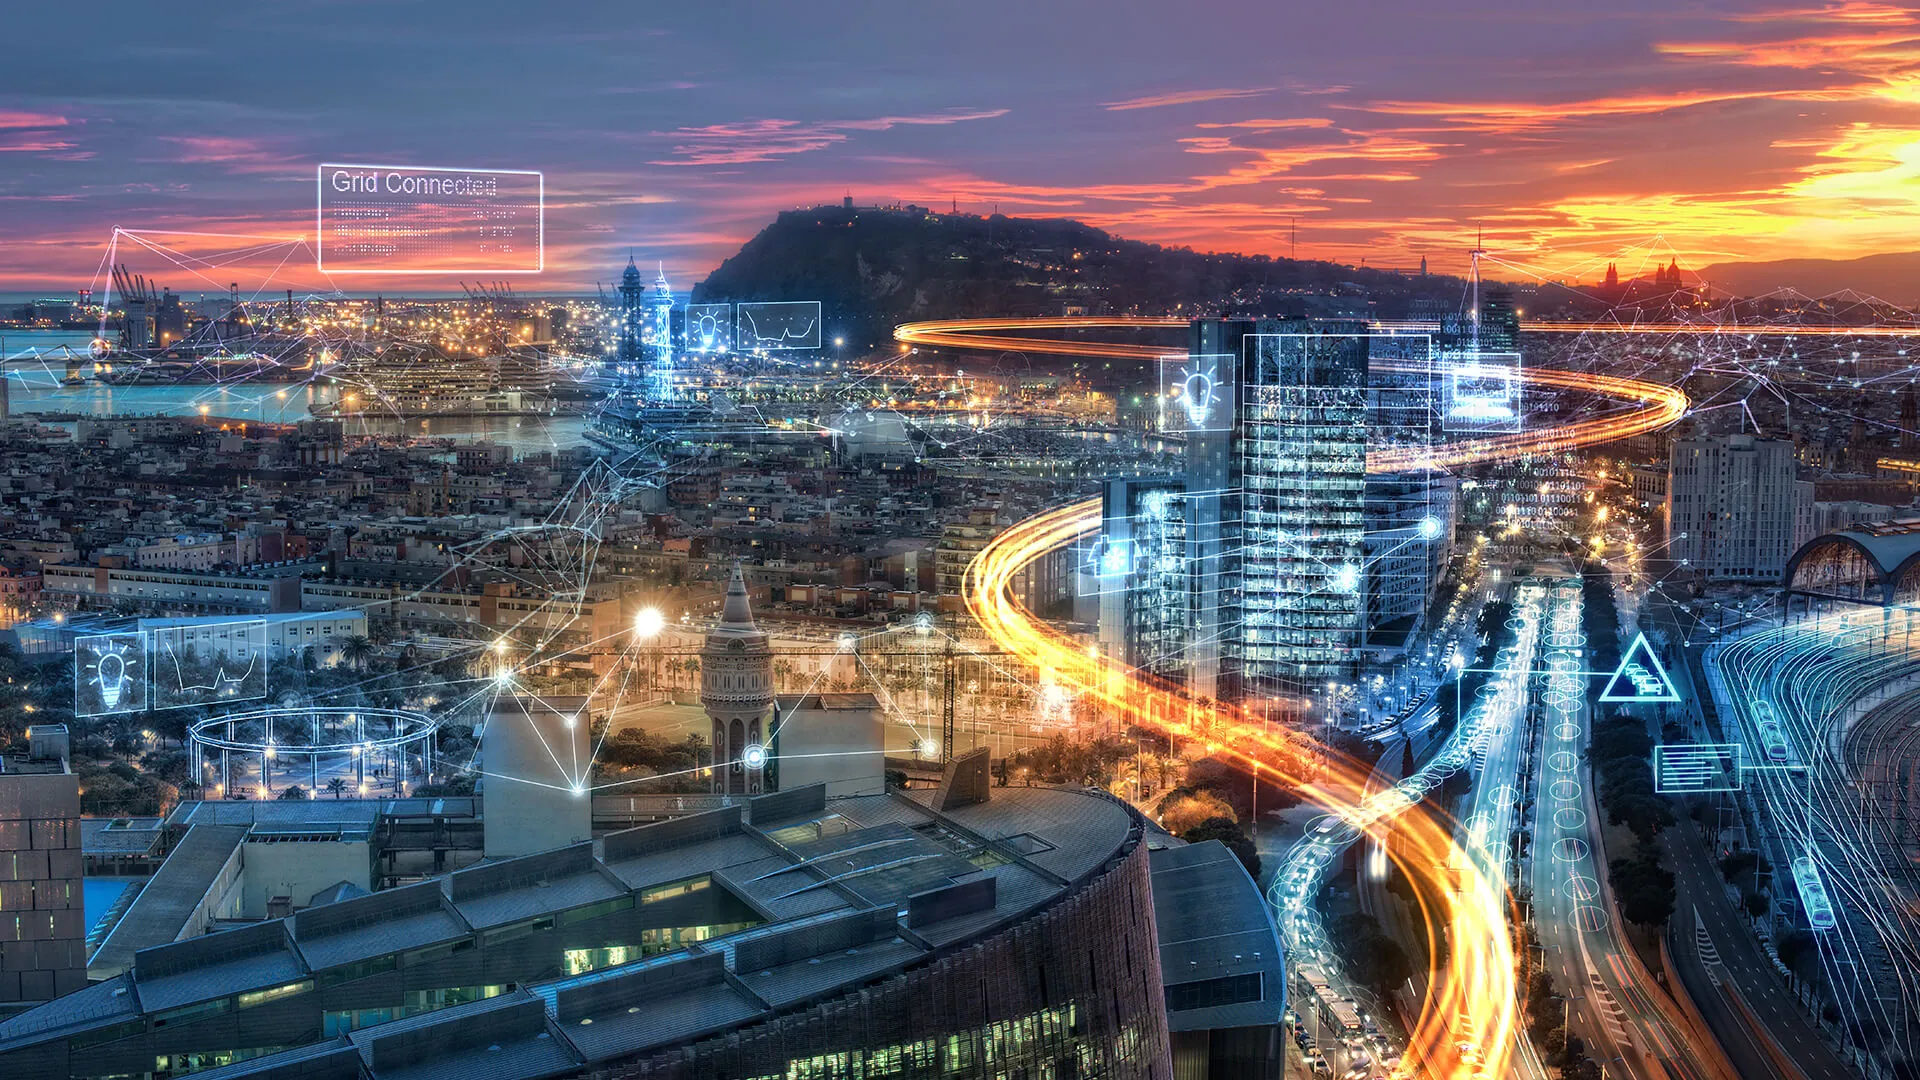
\includegraphics[width=\textwidth]{smartcity.png}}
				\caption*{\textit{Smart City}}
			\end{subfigure}
	\end{figure}
\end{frame}

\setbeamertemplate{background} 
{
	\includegraphics[width=\paperwidth,height=\paperheight]{thank-you.jpg}
}
\begin{frame}[plain]
\end{frame}